\section{Pulsar Magnetosphere}

The basic picture of a pulsar magnetosphere was first presented in
\cite{goldreich_1969_pulsar-electrodynamics}.  The magnetic dipole
of the rotating \ac{NS} creates a quadrupole electric field.

The potential generated
by this field is given as \citep{goldreich_1969_pulsar-electrodynamics}:
\begin{equation}
\PulsarPotential = \frac{\MagneticField \angularfrequency^2 \PulsarRadius^2}{2c^2}
\approx 6\times 10^{12} 
\left(\frac{\MagneticField}{10^{12}\unitspace\gauss}\right)
\left(\frac{\PulsarRadius}{10\unitspace\km}\right)^3
\left(\frac{\period}{1\unitspace\second}\right).
\end{equation}
For \acp{NS}, this potential produces magnetic field is much larger than
the gravitaional force. Threfore, \ac{NS} magnetospheres can act as a
powerful particle accelerators.



\begin{figure}[htpb]
  \begin{center}
    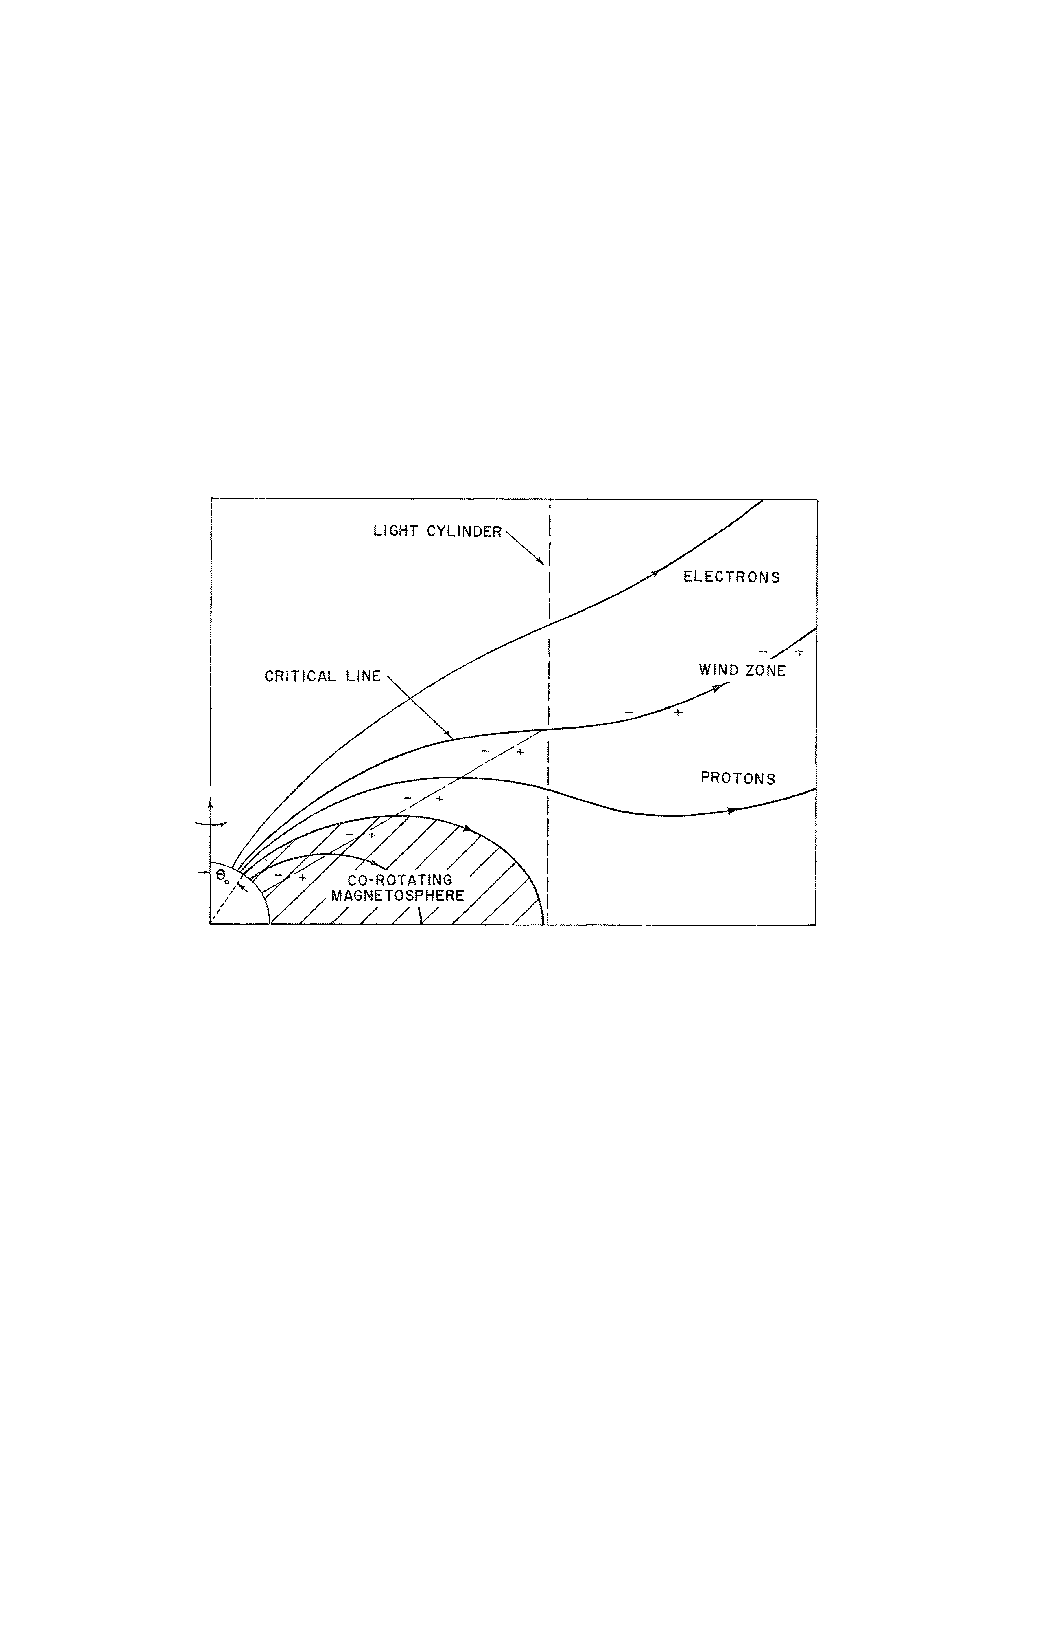
\includegraphics{chapters/pulsar_pwn_system/figures/pulsar_magnetosphere.pdf}
  \end{center}
  \caption{The magnetosphere for a rotating pulsar.
  The pulsar is on the bottom left of the plot. This figure is
  from \cite{goldreich_1969_pulsar-electrodynamics}.}
  \figlabel{pulsar_magnetosphere}
\end{figure}

\figref{pulsar_magnetosphere} shows a schematic diagram of this
magnetosphere.

\begin{itemize}
  \item
    \todo[inline]{Where are sites of acceleratoin}
\item Charge density in magnetosphere?
  \item Radio emission
  \item gamma-ray emission. Slot-gap, outer gap models
"A long standing question in pulsar astronomy has been the location
of the radio emission. Three places have been suggested; near the light
cylinder (Smith 1969), perhaps located in regions of closed magnetic
field lines (Gold 1968), and the open field line regions (Radhakrishnan
\& Cooke 1969). Nowadays, it is widely accepted (see e.g. Lyne \& Smith
1990) that the radio emission originates from the open field line region
well inside the light cylinder, whereas the very high energy emission
(opti- cal and above) probably arises in a quite different mechanism,
much nearer to the light cylinder." -- kramer\_1997a\_origin-pulsar
\end{itemize}


Pulsars typically release only a small percent of their overall
energy budget as pulsed emission. The efficiency of converting
spin-down energy into pulsed $\gamma-$rays is typically $\sim$
0.1\% to 10\% (\cite{abdo_2010a_first-fermi}).  For example, the
Crab nebulae is estimated to release 0.1\% of it's spin-down energy
as pulsed $\gamma$-rays \cite{abdo_2010a_fermi-large}.  Typically,
the energy released as radio and optical photons is much less.
The optical flux of the Crab is a factor of $\sim100$ smaller
\cite{cocke_1969_discovery-optical} and the radio flux is a factor of
$\sim 10^4$ smaller.  
Therefore, the vast majority of the energy output of
the pulsar is carried away as a pulsar wind, which will 
be described in the next section.

